\chapter{Introducción}

A partir del análisis de sentimiento se generaron hiperparámetros de clasificación, correspondientes a pesos asignados de acuerdo a las palabras negativas o positivas identificadas, así como una composición de adjetivos que reflejen objetividad o subjetividad en las expresiones lingüísticas.\\

Esta información nos es de utilidad ya que podemos conocer el sentimiento de respuesta general del publico en sus comentarios, ver el tipo de reacción que tiene sobre el publico, e incluso podría permitir la clasificación del publico objetivo, así como temas de discusión o o identificar comportamiento negativo.\\

\chapter{Descripción de los datos}

Para este reporte se emplean los comentarios en vivo, aportados por usuarios de YouTube durante el primer debate presidencial de México 2024, tal como lo observamos en los reportes anteriores.

\begin{figure}[!h]
	\centering
	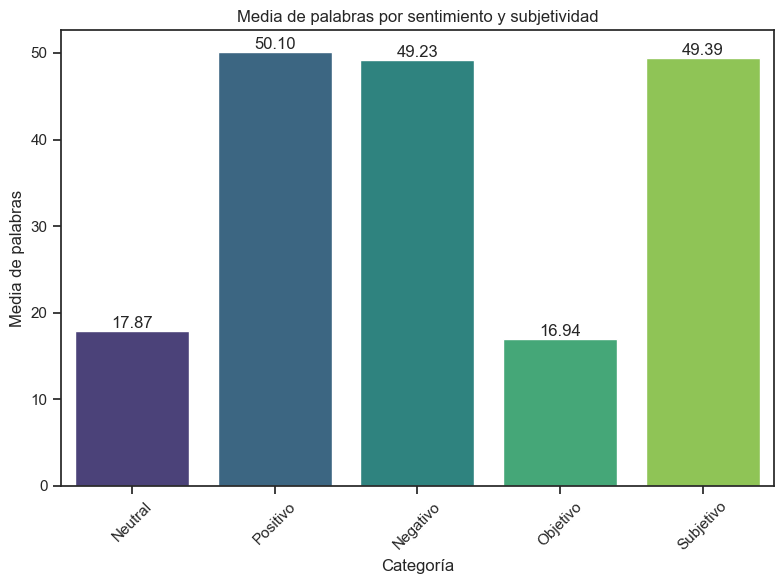
\includegraphics[width=10cm]{Images/Promedio_de_palabras}
	\caption{Distribución de promedio de palabras por sentimiento y objetividad.}
	\label{fig:promediodepalabras}
\end{figure}

Del conjunto de datos, al procesar y clasificar las respuestas del análisis de sentimiento y subjetividad, se realiza la clasificación de los comentarios con base en el valor obtenido de cada escala para cada parámetro, por lo que podemos clasificar los comentarios en 5 tipos distintos; clasificando los comentarios con sentimiento: positivo, neutral y negativo; 2 clasificaciones para comentarios con postura: objetiva y subjetiva. (ver figura \ref{fig:promediodepalabras})\\

A partir de este patrón se infiere una relación entre el tipo de comentario y la extensión de los mismos, observando una mayor expresión de animo y justificación de sentimientos,en el otro extremo, se observa que los comentarios neutrales y objetivos contienen significativamente una media de menor palabras en comparación con los comentarios positivos, negativos y subjetivos en donde se identifica un conteo alto de palabras, podemos observar esta misma distribución en el conteo de caracteres (ver figura \ref{fig:promediodecaracteres}).

\begin{figure}[!h]
	\centering
	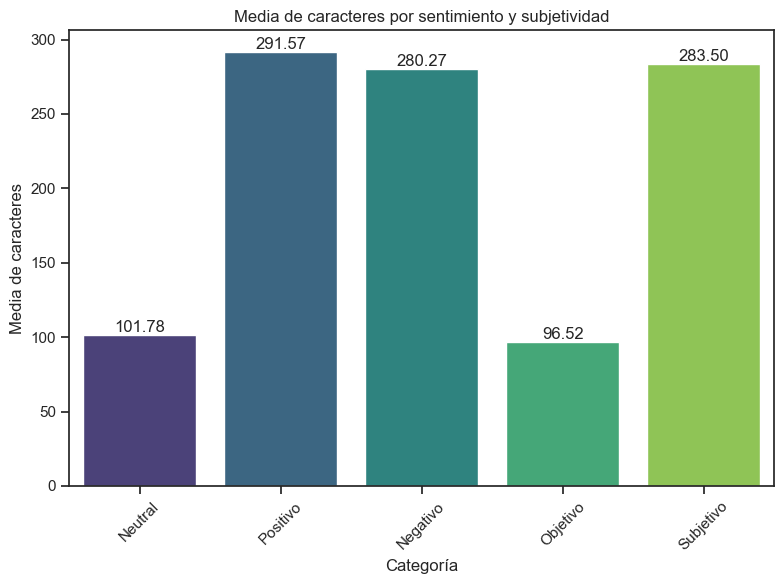
\includegraphics[width=10cm]{Images/Promedio_de_caracteres}
	\caption{Distribución de promedio de caracteres por sentimiento y objetividad.}
	\label{fig:promediodecaracteres}
\end{figure}

Al realizar el análisis del de densidad por atributos o clasificación, se identifica una diferencia significativa mayor de comentarios con un sentimiento neutral, a diferencia de aquellos positivos o negativos, estos últimos se presentan un numero significativamente menor, lo que se puede inferir como una respuesta mas concienzuda del publico respecto a sus comentarios en el video del debate, siendo mayor la densidad de comentarios con un sentimiento positivo en comparación con aquellos con una connotación negativa \ref{fig:DDSN}.
\clearpage
\begin{figure}[!h]
	\centering
	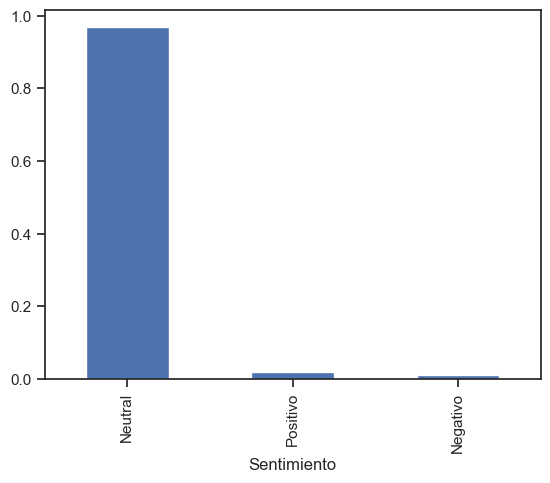
\includegraphics[width=10cm]{Images/Densidad_sentimientos}
	\caption{Distribución de densidad de sentimientos Normalizada.}
	\label{fig:DDSN}
\end{figure}

En la distribución de densidad de subjetividad presenta una mayor densidad de comentarios de atributo objetivo que aquellos subjetivos, lo que puede indicar una tendencia alta de comentarios objetivos que subjetivos (ver figura\ref{fig:DDSbN}).\\


\begin{figure}[!h]
	\centering
	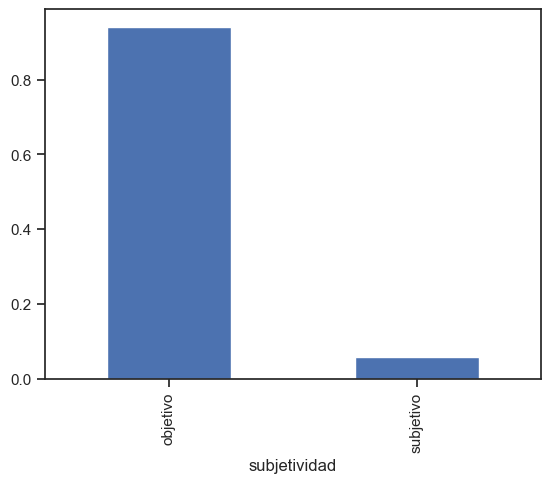
\includegraphics[width=10cm]{Images/Densidad_subjetividad}
	\caption{Distribución de densidad de subjetividad Normalizada.}
	\label{fig:DDSbN}
\end{figure}

Mientras que al comparar la distribución del conteo de palabras con sentimiento, positivo, neutral y negativo, se observa que las palabras de carácter neutral presentan una distribución exponencial, esta misma distribución se observa en las palabras con sentimientos positivos y negativos, sin embargo estas ultimas presentan una distribución mas dispersas y en menor densidad al compararlas con las neutrales.

\begin{figure}[!h]
	\centering
	\includegraphics[width=10cm]{Images/Palabras_sentimiento}
	\caption{Conteo de palabras y su parámetro de sentimiento.}
	\label{fig:CPPS}
\end{figure}

Al analizar la distribución del conteo de palabras objetivas y subjetivas se observa una distribución exponencial, al igual que el grafico anterior, la distribución se concentra en bajos conteos de palabras objetivas, lo que indica un patrón entre la neutralidad y la objetividad de los comentarios (ver figura \ref{fig:CPPo}). 

\begin{figure}[!h]
	\centering
	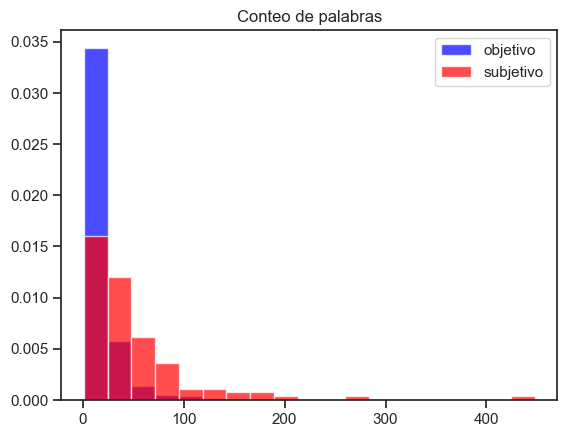
\includegraphics[width=10cm]{Images/Palabras_objetividad}
	\caption{Conteo de palabras y su parámetro de objetividad.}
	\label{fig:CPPo}
\end{figure}
\chapter{Conclusiones}

A partir de los resultados y las observaciones realizadas al comparar los modelos y sus hiperparámetros, se concluye que los comentarios neutrales y objetivos tiene una alta correlación en su distribución, esta efecto se observa en las figuras \ref{fig:promediodepalabras} y \ref{fig:promediodecaracteres}, en las cuales se observa una distribución similar de conteo de palabras en ambos casos.\\

Mediante el análisis de la densidad de palabras por sentimiento y objetividad, podemos caracterizar claramente la el sentir general de los comentarios, al clasificarlos se observa una marcada tendencia a la neutralidad y objetividad, de esto se infiere que la mayor parte de los comentarios presentan objetividad y neutralidad en sus comentarios.\\

En general se puede concluir que mientras el apoyo en los comentarios esta de lado de Claudia sheinbaum, los comentarios que reflejan esta tendencia son en su mayoría con un apoyo objetivo y no basada en sentimentalismos, esto podría indicar una lección mas consiente o un apoyo mas consciente hacia este candidato.\\



